\documentclass[margin=2mm]{standalone}
\usepackage{tikz}
\usetikzlibrary{calc,positioning,shapes.geometric,backgrounds,fit,shadows.blur,arrows,arrows.meta,decorations.markings}
\tikzset{
  hole/.style = {fill = #1, circle, minimum width = 2.5mm, inner sep = 0mm},
  wire/.style = {draw = #1, line width = .5mm},
  label/.style = {black!50!white, font=\sffamily, anchor = center},
  text/.style = {white, font=\sffamily, anchor = right},
}
\begin{document}
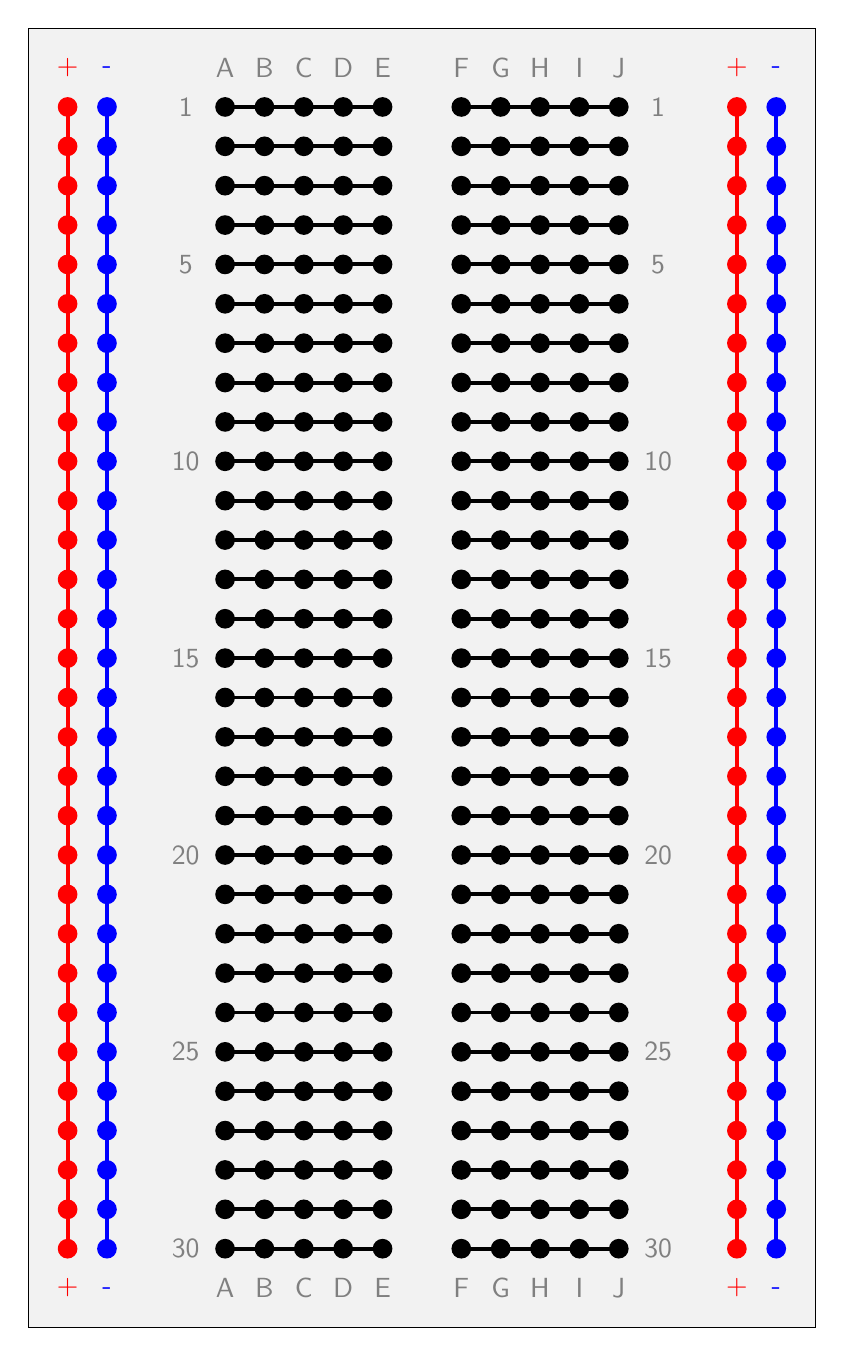
\begin{tikzpicture}[x= 5mm,y=5mm]
% breadboard
  \draw[fill=black!05!white] (-4,-1) rectangle (16,32);
  \draw[wire=red]  (-3,1) -- (-3,30);
  \draw[wire=blue] (-2,1) -- (-2,30);
  \draw[wire=red]  (14,1) -- (14,30);
  \draw[wire=blue] (15,1) -- (15,30);
  \foreach \yi in {1,...,30}{
    \node[hole=red]  at (-3,\yi){};
    \node[hole=blue] at (-2,\yi){};
    \node[hole=red]  at (14,\yi){};
    \node[hole=blue] at (15,\yi){};
    \foreach \xs in {0,6}{
      \draw[wire=black] (\xs+1,\yi) -- (\xs+5,\yi);
      \foreach \xi in {1,2,3,4,5}{
        \node[hole=black] at (\xi+\xs,\yi){};
      }
    }
  }
  \foreach \m/\xi in {A/1,B/2,C/3,D/4,E/5,F/7,G/8,H/9,I/10,J/11}{
    \node[label=90] at (\xi,0) {\m};
    \node[label=90] at (\xi,31) {\m};
  }
  \foreach \m/\yi in {30/1,25/6,20/11,15/16,10/21,5/26,1/30}{
    \node[label=90] at (0,\yi) {\m};
    \node[label=90] at (12,\yi) {\m};
  }
  \foreach \m/\xi in {+/-3,+/14}{
    \node[red] at (\xi,0) {\m};
    \node[red] at (\xi,31) {\m};
  }
  \foreach \m/\xi in {-/-2,-/15}{
    \node[blue] at (\xi,0) {\m};
    \node[blue] at (\xi,31) {\m};
  }
\end{tikzpicture}
\end{document}